\documentclass[a4paper,12pt]{article}
\usepackage{amsmath}
\usepackage{graphicx}
\begin{document}
\title{Homework 3}
\author{Matt Forbes}
\date{October 19, 2010}
\maketitle
\section*{Problem 3.8}
\subsection*{a\()\)}
\begin{center}
  \begin{tabular}{| c | c c c c |}
    \hline
    0 & 2 & -1 & 1 & 1 \\
    \hline
    5 & 1 & 2 & 0 & -1 \\
    10 & -1 & 1 & -2 & 1 \\
    \hline
  \end{tabular}
\end{center}
Pivots to:
\begin{center}
  \begin{tabular}{| c | c c c c |}
    \hline
    15 & 0 & 0 & \(-\frac{7}{3}\) & 3 \\
    \hline
    (-5) & 1 & 0 & \(\frac{4}{3}\) & -1 \\
    5 & 0 & 1 & \(-\frac{2}{3}\) & 0 \\
    \hline
  \end{tabular}
\end{center}
Subproblem on row 2 gives:
\begin{center}
  \begin{tabular}{| c | c c c c |}
    \hline
    0 & 3 & 0 & \(\frac{5}{3}\) & 0 \\
    \hline
    5 & -1 & 0 & \(-\frac{4}{3}\) & 1 \\
    5 & 0 & 1 & \(-\frac{2}{3}\) & 0 \\
    \hline
  \end{tabular}
\end{center}
Which is in optimal form giving {\bf x} = \( (0 \quad 5 \quad 0 \quad  5)^T \)
\subsection*{b\()\)}
\begin{center}
  \begin{tabular}{| c | c c c c |}
    \hline
    0 & 2 & -1 & 1 & 1 \\
    \hline
    5 & 1 & 2 & 0 & -1 \\
    10 & -1 & 1 & -2 & 1 \\
    \hline
  \end{tabular}
\end{center}
In artificial problem form:
\begin{center}
  \begin{tabular}{| c | c c c c c c |}
    \hline
    0 & 0 & 0 & 0 & 0 & 1 & 1 \\
    \hline
    5 & 1 & 2 & 0 & -1 & 1 & 0 \\
    10 & -1 & 1 & -2 & 1 & 0 & 1 \\
    \hline
  \end{tabular}
\end{center}
Which pivots to:
\begin{center}
  \begin{tabular}{| c | c c c c c c |}
    \hline
    0 & 0 & 0 & 0 & 0 & \(\frac{1}{2}\) & 1 \\
    \hline
    5 & 0 & 1 & \(-\frac{2}{3}\) & 0 & \(\frac{1}{3}\) & \(\frac{1}{3}\) \\
    5 & -1 & 0 & \(-\frac{4}{3}\) & 1 & \(-\frac{1}{3}\) & \(\frac{2}{3}\) \\
    \hline
  \end{tabular}
\end{center}
This artificial problem's minimum is 0, so the original is feasible: Reformulate:
\begin{center}
  \begin{tabular}{| c | c c c c |}
    \hline
    0 & 2 & -1 & 1 & 1 \\
    \hline
    5 & 0 & 1 & \(-\frac{2}{3}\) & 0 \\
    5 & -1 & 0 & \(-\frac{4}{3}\) & 1 \\
    \hline
  \end{tabular}
\end{center}
Pivots to:
\begin{center}
  \begin{tabular}{| c | c c c c |}
    \hline
    0 & 3 & 0 & \(\frac{5}{3}\) & 0 \\
    \hline
    5 & -1 & 0 & \(-\frac{4}{3}\) & 1 \\
    5 & 0 & 1 & \(-\frac{2}{3}\) & 0 \\
    \hline
  \end{tabular}
\end{center}
Which is in optimal form giving {\bf x} = \( (0 \quad 5 \quad 0 \quad  5)^T \)
\section*{Problem 3.15}
This problem formulated using \(|D_i| = D_i^+ + D_i^-\) is:
\begin{alignat*}{10}
  \min \quad {}& {}& {}& {}& D_1^+& + D_1^-& + D_2^+& + D_2^-& + D_3^+& + D_3^-& + D_4^+& + D_4^-& \\
  \text{s. t.} \quad 5& = a& + b& +c& -D_1^+& + D_1^-& {}& {}& {}& {}& {}& {}& \\ 
  13& = 4a& + 2b& + c& {}& {}& - D_2^+& + D_2^-& {}& {}& {}& {}&\\
  30& = 16a& + 4b& + c& {}& {}& {}& {}& - D_3^+& + D_3^-& {}& {}&\\
  45& = 25a& + 5b& + c& {}& {}& {}& {}& {}& {}& - D_4^+& - D_4^-&
\end{alignat*}
Which has the simplex tableau of:
\begin{center}
\begin{tabular}{| c | c  c  c  c  c  c  c  c  c  c  c |}
\hline
0 & 0 & 0 & 0 & 1 & 1 & 1 & 1 & 1 & 1 & 1 & 1\\
\hline
5 & 1 & 1 & 1 & -1 & 1 & 0 & 0 & 0 & 0 & 0 & 0\\
13 & 4 & 2 & 1 & 0 & 0 & -1 & 1 & 0 & 0 & 0 & 0\\
30 & 16 & 4 & 1 & 0 & 0 & 0 & 0 & -1 & 1 & 0 & 0\\
45 & 25 & 5 & 1 & 0 & 0 & 0 & 0 & 0 & 0 & -1 & 1\\
\hline
\end{tabular}
\end{center}
Pivots to:
\begin{center}
\begin{tabular}{| c | c  c  c  c  c  c  c  c  c  c  c |}
\hline
-93 & -46 & -12 & -4 & 2 & 0 & 2 & 0 & 2 & 0 & 2 & 0\\
\hline
5 & 1 & 1 & 1 & -1 & 1 & 0 & 0 & 0 & 0 & 0 & 0\\
13 & 4 & 2 & 1 & 0 & 0 & -1 & 1 & 0 & 0 & 0 & 0\\
30 & 16 & 4 & 1 & 0 & 0 & 0 & 0 & -1 & 1 & 0 & 0\\
45 & 25 & 5 & 1 & 0 & 0 & 0 & 0 & 0 & 0 & -1 & 1\\
\hline
\end{tabular}
\end{center}
Which is now in canonical form. Now using successive ratio rules for pivoting:
\begin{center}
\begin{tabular}{| c | c  c  c  c  c  c  c  c  c  c  c |}
\hline
-10.2 & 0 & -2.8 & -2.16 & 2 & 0 & 2 & 0 & 2 & 0 & 0.16 & 1.84\\
\hline
3.2 & 0 & 0.8 & 0.96 & -1 & 1 & 0 & 0 & 0 & 0 & 0.04 & -0.04\\
5.8 & 0 & 1.2 & 0.84 & 0 & 0 & -1 & 1 & 0 & 0 & 0.16 & -0.16\\
1.2 & 0 & 0.8 & 0.36 & 0 & 0 & 0 & 0 & -1 & 1 & 0.64 & -0.64\\
1.8 & 1 & 0.2 & 0.04 & 0 & 0 & 0 & 0 & 0 & 0 & -0.04 & 0.04\\
\hline
\end{tabular}
\end{center}
Again:
\begin{center}
\begin{tabular}{| c | c  c  c  c  c  c  c  c  c  c  c |}
\hline
-6 & 0 & 0 & -0.9 & 2 & 0 & 2 & 0 & -1.5 & 3.5 & 2.4 & -0.4\\
\hline
2 & 0 & 0 & 0.6 & -1 & 1 & 0 & 0 & 1 & -1 & -0.6 & 0.6\\
4 & 0 & 0 & 0.3 & 0 & 0 & -1 & 1 & 1.5 & -1.5 & -0.8 & 0.8\\
1.5 & 0 & 1 & 0.45 & 0 & 0 & 0 & 0 & -1.25 & 1.25 & 0.8 & -0.8\\
1.5 & 1 & 0 & -0.05 & 0 & 0 & 0 & 0 & 0.25 & -0.25 & -0.2 & 0.2\\
\hline
\end{tabular}
\end{center}
And finally:
\begin{center}
\begin{tabular}{| c | c  c  c  c  c  c  c  c  c  c  c |}
\hline
-3 & 0 & 0 & 0 & 0.5 & 1.5 & 2 & 0 & 0 & 2 & 1.5 & 0.5\\
\hline
3.33333 & 0 & 0 & 1 & -1.66667 & 1.66667 & 0 & 0 & 1.66667 & -1.66667 & -1 & 1\\
3 & 0 & 0 & 0 & 0.5 & -0.5 & -1 & 1 & 1 & -1 & -0.5 & 0.5\\
0 & 0 & 1 & 0 & 0.75 & -0.75 & 0 & 0 & -2 & 2 & 1.25 & -1.25\\
1.66667 & 1 & 0 & 0 & -0.0833333 & 0.0833333 & 0 & 0 & 0.333333 & -0.333333 & -0.25 & 0.25\\
\hline
\end{tabular}
\end{center}
This gives values: \(a=\frac{5}{3}, b=0, c=\frac{10}{3} \)\\
Here is a graph of the fit curve vs actual points: \\
\begin{center}
  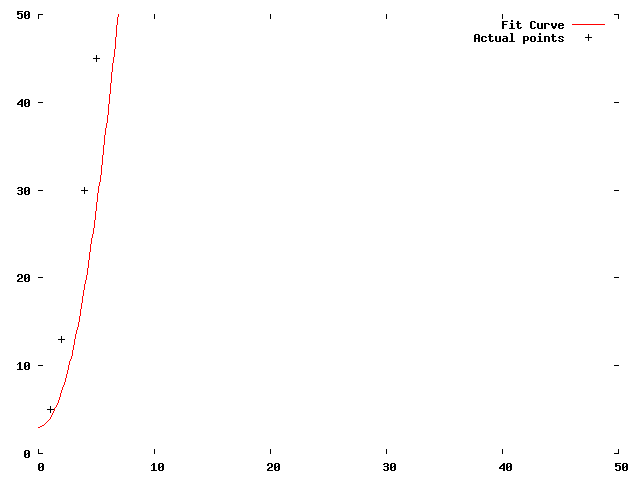
\includegraphics[width=10cm, height=10cm, keepaspectratio=true]{315.png}
\end{center}
\section*{Problem 3.16}
\subsection*{a\()\)}
\begin{center}
\begin{tabular}{| c | c  c  c  c  c |}
\hline
3 & 1 & 0 & 0 & 1 & 0\\
\hline
-1 & 1 & 1 & 0 & -1 & 0\\
-4 & -1 & 0 & 1 & -1 & 0\\
1 & 1 & 0 & 0 & 0 & 1\\
\hline
\end{tabular}
\end{center}
Pivots to:
\begin{center}
\begin{tabular}{| c | c  c  c  c  c |}
\hline
2 & 0 & 0 & 0 & 1 & -1\\
\hline
-2 & 0 & 1 & 0 & -1 & -1\\
-3 & 0 & 0 & 1 & -1 & 1\\
1 & 1 & 0 & 0 & 0 & 1\\
\hline
\end{tabular}
\end{center}
And in optimal form:
\begin{center}
\begin{tabular}{| c | c  c  c  c  c |}
\hline
-1 & 0 & 0 & 1 & 0 & 0\\
\hline
1 & 0 & 1 & -1 & 0 & -2\\
3 & 0 & 0 & -1 & 1 & -1\\
1 & 1 & 0 & 0 & 0 & 1\\
\hline
\end{tabular}
\end{center}
With solution {\bf x} = \( (1 \quad 1 \quad 0 \quad 3 \quad 0)^T \)
\subsection*{b\()\)}
\begin{center}
\begin{tabular}{| c | c  c  c  c  c |}
\hline
-1 & 0 & 0 & -1 & 0 & 1\\
\hline
-1 & 1 & 0 & 0 & 2 & -1\\
-1 & 0 & 0 & 1 & 1 & -1\\
-2 & -3 & 1 & 5 & 0 & -2\\
\hline
\end{tabular}
\end{center}
Pivots to:
\begin{center}
\begin{tabular}{| c | c  c  c  c  c |}
\hline
-2 & 1 & 0 & -1 & 2 & 0\\
\hline
1 & -1 & 0 & 0 & -2 & 1\\
0 & -1 & 0 & 1 & -1 & 0\\
0 & -5 & 1 & 5 & -4 & 0\\
\hline
\end{tabular}
\end{center}
And in optimal form:
\begin{center}
\begin{tabular}{| c | c  c  c  c  c |}
\hline
-2 & 0 & 0 & 0 & 1 & 0\\
\hline
1 & -1 & 0 & 0 & -2 & 1\\
0 & -1 & 0 & 1 & -1 & 0\\
0 & 0 & 1 & 0 & 1 & 0\\
\hline
\end{tabular}
\end{center}
With solution {\bf x} = \( (0 \quad 0 \quad 0 \quad 0 \quad 1)^T \)
\subsection*{c\()\)}
This tableau is already in optimal form:
\begin{center}
\begin{tabular}{| c | c  c  c  c  c  c |}
\hline
0 & 2 & 5 & 3 & 0 & 0 & 0\\
\hline
5 & 1 & 1 & 0 & 1 & 0 & 0\\
15 & 2 & 1 & 2 & 0 & 1 & 0\\
8 & 1 & 1 & 1 & 0 & 0 & 1\\
\hline
\end{tabular}
\end{center}
With solution {\bf x} = \( (0 \quad 0 \quad 0 \quad 0 \quad 5 \quad 15 \quad 8)^T \)
\section*{Problem 3.17}
Original Problem:
\begin{alignat*}{5}
  \min \quad x_1& + 2x_2& - x_3& {}&\\
  \text{s. t.} \quad x_1& - x_2& + x_3& \le 1\\
  x_1& + x_2& - 2x_3& \le 4\\
  x_1 \ge 0& , x_2, x_3& \text{ free}
\end{alignat*}
Reformulated with slack variables, and: \(x_2 = (x_2' - x_2''), x_3 = (x_3' - x_3'')\):
\begin{alignat*}{8}
  \min \quad x_1& + 2x_2'& -2x_2''& - x_3'& + x_3''& {}& {}& {}&\\
  \text{s.t.} \quad x_1& - x_2'& + x_2''& + x_3'& - x_3''& + x_4& {}& = 1\\
  x_1& + x_2'& - x_2''& - 2x_3'& + 2x_3''& {}& + x_5& = 4
\end{alignat*}
Has the simplex tableau:
\begin{center}
\begin{tabular}{| c | c  c  c  c  c  c  c |}
\hline
0 & 1 & 2 & -2 & -1 & 1 & 0 & 0\\
\hline
1 & 1 & -1 & 1 & 1 & -1 & 1 & 0\\
4 & 1 & 1 & -1 & -2 & 2 & 0 & 1\\
\hline
\end{tabular}
\end{center}
Pivots to:
\begin{center}
\begin{tabular}{| c | c  c  c  c  c  c  c |}
\hline
2 & 3 & 0 & 0 & 1 & -1 & 2 & 0\\
\hline
1 & 1 & -1 & 1 & 1 & -1 & 1 & 0\\
5 & 2 & 0 & 0 & -1 & 1 & 1 & 1\\
\hline
\end{tabular}
\end{center}
And in optimal form:
\begin{center}
\begin{tabular}{| c | c  c  c  c  c  c  c |}
\hline
7 & 5 & 0 & 0 & 0 & 0 & 3 & 1\\
\hline
6 & 3 & -1 & 1 & 0 & 0 & 2 & 1\\
5 & 2 & 0 & 0 & -1 & 1 & 1 & 1\\
\hline
\end{tabular}
\end{center}
With solution {\bf x} = \( (0 \quad 0 \quad 6 \quad 0 \quad 5 \quad 0 \quad 0)^T\)\\
Resubstituting \(x_2 = x_2' - x_2''\) and \(x_3 = x_3' - x_3''\) gives this solution
to the original problem: \( (0 \quad -6 \quad -5)^T \)
\section*{Problem 3.19}
Reformulating the system of equations into an artificial problem
will show whether or not it has any feasible solution.
\begin{center}
\begin{tabular}{| c | c  c  c  c  c  c  c  c  c  c |}
\hline
0 & 0 & 0 & 0 & 0 & 0 & 0 & 0 & 1 & 1 & 1\\
\hline
-1 & 1 & 1 & 0 & -1 & 1 & 0 & 0 & 1 & 0 & 0\\
1 & -1 & 0 & 1 & 1 & 0 & 1 & 0 & 0 & 1 & 0\\
-1 & 0 & 1 & -1 & 0 & 0 & 0 & 1 & 0 & 0 & 1\\
\hline
\end{tabular}
\end{center}
Pivoting using subproblem (obj function row 1):
\begin{center}
\begin{tabular}{| c | c  c  c  c  c  c  c  c  c  c |}
\hline
0 & 0 & 0 & 0 & 0 & 0 & 0 & 0 & 1 & 1 & 1\\
\hline
0 & 0 & 1 & 1 & 0 & 1 & 1 & 0 & 1 & 1 & 0\\
1 & -1 & 0 & 1 & 1 & 0 & 1 & 0 & 0 & 1 & 0\\
-1 & 0 & 1 & -1 & 0 & 0 & 0 & 1 & 0 & 0 & 1\\
\hline
\end{tabular}
\end{center}
Again pivoting with a subproblem (obj function row3)
\begin{center}
\begin{tabular}{| c | c  c  c  c  c  c  c  c  c  c |}
\hline
0 & 0 & 0 & 0 & 0 & 0 & 0 & 0 & 1 & 1 & 1\\
\hline
0 & 0 & 1 & 1 & 0 & 1 & 1 & 0 & 1 & 1 & 0\\
1 & -1 & -1 & 0 & 1 & -1 & 0 & 0 & -1 & 0 & 0\\
-1 & 0 & 2 & 0 & 0 & 1 & 1 & 1 & 1 & 1 & 1\\
\hline
\end{tabular}
\end{center}
This tableau is in infeasible form 2. The system has no solution.
\section*{Problem 3.21}
This problem calls for minimizing the max (minimax) of two expressions. This is not a linear
objective function, but can be reformulated as such. If we create some free variable w and constrain
it to being greater than both expressions, then finding the minimum value of w will also be the
smallest max of the two expressions.\\\\
w is a free variable so we can write it as \(w = w' - w''\) and then constrain \( w', w'' \ge 0 \).\\\\
In standard form (with slack variables):
\begin{alignat*}{7}
  \min \quad w'& - w''& {}& {}& {}& {}& {}& {}&\\
  \text{s.t.} -w'& + w''& + 2x_1& - x_2& + x_3& {}& {}& = 0\\
  -w'& + w''& -3x_1& + 2x_2& {}& + x_4& {}& = 0\\
  {}& {}& 4x_1& + x_2& {}& {}& + x_5& = 5\\
\end{alignat*}
The simplex tableau:
\begin{center}
\begin{tabular}{| c | c  c  c  c  c  c  c |}
\hline
0 & 1 & -1 & 0 & 0 & 0 & 0 & 0\\
\hline
0 & -1 & 1 & 2 & -1 & 1 & 0 & 0\\
0 & -1 & 1 & -3 & 2 & 0 & 1 & 0\\
5 & 0 & 0 & 4 & 1 & 0 & 0 & 1\\
\hline
\end{tabular}
\end{center}
Which is already in canonical form, pivoting:
\begin{center}
\begin{tabular}{| c | c  c  c  c  c  c  c |}
\hline
0 & 0 & 0 & 2 & -1 & 1 & 0 & 0\\
\hline
0 & -1 & 1 & 2 & -1 & 1 & 0 & 0\\
0 & 0 & 0 & -5 & 3 & -1 & 1 & 0\\
5 & 0 & 0 & 4 & 1 & 0 & 0 & 1\\
\hline
\end{tabular}
\end{center}
Pivot again for optimal form:
\begin{center}
\begin{tabular}{| c | c  c  c  c  c  c  c |}
\hline
0 & 0 & 0 & 0.333333 & 0 & 0.666667 & 0.333333 & 0\\
\hline
0 & -1 & 1 & 0.333333 & 0 & 0.666667 & 0.333333 & 0\\
0 & 0 & 0 & -1.66667 & 1 & -0.333333 & 0.333333 & 0\\
5 & 0 & 0 & 5.66667 & 0 & 0.333333 & -0.333333 & 1\\
\hline
\end{tabular}
\end{center}
This gives a solution of \( (0 \quad 0 \quad 0 \quad 0 \quad 0 \quad 0 \quad 5)^T \)\\  which means
that \( x_1 = 0, x_2 = 0 \), which is within the constraints and does produce the smallest value
of either expression in the objective function.

\section*{Problem 3.23}
a)True\\b)True\\c)False\\d)True\\e)True\\f)True\\g)False\\i)True
\end{document}

